\chapter{Introduction}
\label{introduction}

As the efficiency and accuracy of rapid genome sequencing skyrockets, the potential for personalized therapies has made its way from science fiction to scientific reality. Using genetics to understand, diagnose, and eventually to predict illness is not a new idea; in recent years, however, technological ability and scientific understanding have advanced to such a point that researchers may predict risk for several diseases with reasonable confidence. Increasingly, variants in the human genome are being identified as being robustly linked to risk for complex illnesses such as heart disease [\small{cite 9p21}], obesity [\small{cite fto}], and schizophrenia [\small{cite something}]. However, much work remains to be done in order to create tools which may accurately predict individual disease risk from known and unknown genetic risk factors. In this thesis, we propose a novel extension to a well known methodology in order to better characterize disease risk from comorbid conditions using only summary statistics. 

In brief, we present preliminary evidence for the use of \ac{PRS}s in predicting \ac{CAD}. We use recently published summary statistics from a \ac{GWAS} conducted by the \ac{CARDIOGRAMC4D} consortium alongside evidence gathered by the \ac{GLC} and the \ac{GIANT} consortium for lipids and \ac{BMI} \textit{per say}. We use this data alongside previously identified variants to construct first a simplistic \ac{PRS} using only genome wide statistically signficant ($P_{Bonferonni} < 0.05$ or $q_{FDR}$ < 0.05) variants, then expand our search to variants which may not be as robustly linked to phenotype. [Cite storey, BH, and dudbridge]. We use an empirical maximation approach and several strategies of mathematical optimization in order to construct an \ac{oPRS}, then devise a novel technique for integrating information from co-morbid \ac{oPRS} diseases in order to better predict \ac{CAD} in four cohorts comprising approximately $n=12,000$ individuals

\section{Genetics of Coronary Artery Disease}

\ac{CAD} occurs when the major blood vessels supplying the heart become diseased or damaged, often leading to severe complications such as \ac{MI} and death. [cite review articles] \ac{CAD} is known to be a complex genetic disease with heritability estimated by twin studies between 40 and 60\%. [mcPherson 2016, twin studies paper] Several important variants have been indentified which have been shown to robustly increase risk to \ac{CAD} by altering lipid transporting pathways [cite LDLR], structural collegan bodies [TRIB 1??], and others factors. 


\begin{figure}[h]
\caption{Progression of the formation of plaque causing \ac{CAD}. Adapted from Gretch 2003.}
\centering
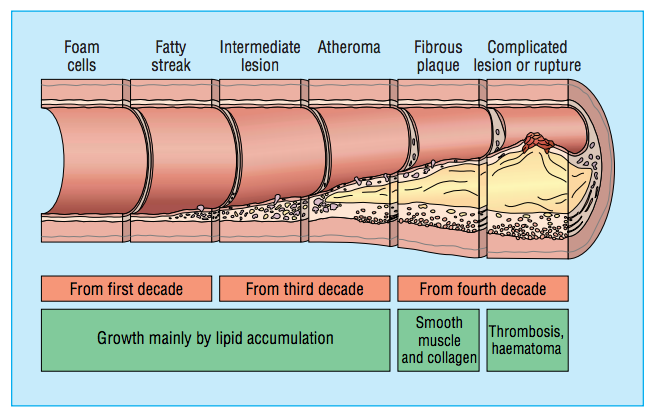
\includegraphics[width=0.8\textwidth]{Figures/cad.png}
\end{figure}

With heart disease and stroke the leading cause of perscription drug use in Canada as well as one of the leading causes of death and hospitalization [cite herat and stroke], the need to better understand, diagnose, and prevent this deadly disease is apparent.  In order to better understand the need for improved statistical methodologies, it is important to understand the large body of previous attempts to characterize the genetic determinants of \ac{CAD}

Despite some promising beginings, initial attempts to understand and explain \ac{CAD} through genetics were largely unsuccessful.[CITE] The first variant to be succesfully and robustly linked to risk for \ac{CAD} was the 9p21.3 locus. Discovered by a team of researchers at the Univeristy of Ottawa Heart institute, the allele consists of a 58 \ac{kb} region on chromosome 9 which was shown to be associated with \ac{CAD} in a population of 23,000 caucasion individuals. (\cite{McPherson2016})

\begin{figure}[h]
\caption{Fine mapping of the genomic interval on chromosome 9 associated with Coronary Heart Disease. Adapted from Mcpherson et al 2006}
\centering
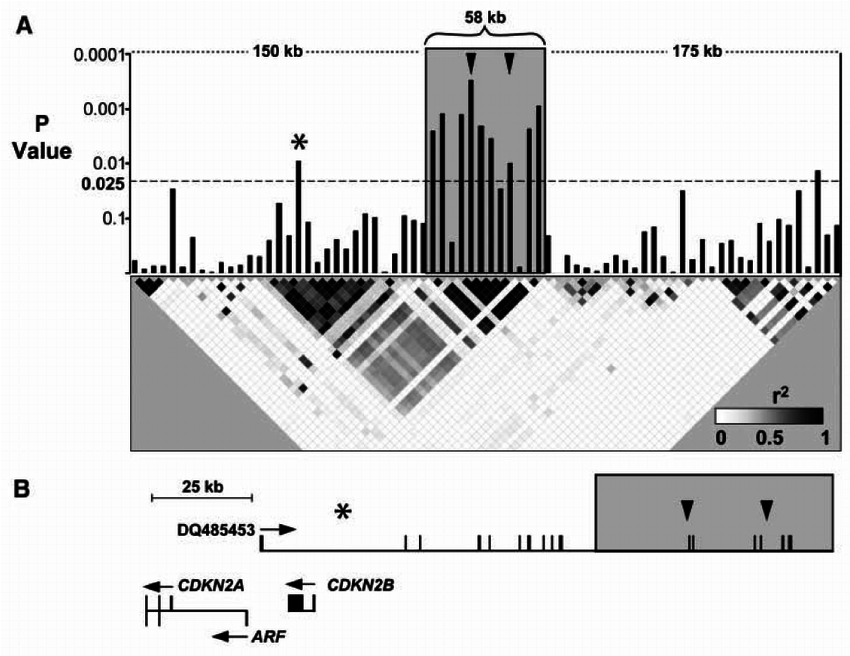
\includegraphics[width=0.8\textwidth]{Figures/9p21.png}
\end{figure}

This initial success began the era of the \ac{GWAS}, explained in more detail in section \ref{gwas}.  Researchers across the globe began frantically searching for more loci with the hope of understanding and predicting complex disease; in that goal, the \ac{GWAS} has failed. (\cite{Visscher2012}) A number of important genetic markers for \ac{CAD} have been discovered, but often in small familial cases or with very low effect sizes. [Cite] As the dust settles and the low hanging fruit have been picked, common variants have been shown to explain approximately 28\% of the heritablity of \ac{CAD} [cite majid], yet a large portion remains to be accounted for. This has become known as the problem of ``missing heritabillity'' of complex disease; common genetic variants explain a relatively small portion of the total estimated heritability of a disease, therefore researchers must resort to ever more obscure and complex methods to attempt to explain the complex interactions between genetic elements in the human genome. [cite review paper] From pathway analysis to partitioned heritability to all kinds of arcane statistical procedures, researchers from across the globe have tried their hardest to shrink this gap between our knowledge and accurate prediction and understanding of complex disease. To this end, we develop our own methodology incorporating multiple sources of information for the more accurate prediction of clinical end points. 

\section{Genome Wide Association Studies} \label{gwas}

In order to properly introduce the model, however, the basic underpinnings must be explored and explained. Genome wide association studies seek to indetify associations between individual genotypes and disease phenotypes in a hypothesis free manner. In this section, the statistical model required to understand \ac{GWAS} is presented and explored.

\subsection{Primer on Genetics}

\ac{DNA} is a double helical molecule which encodes the genetic blueprints for the construction of proteins and other materials that make up every known living organism. \ac{DNA} is composed of three parts: a negatively charged phosphate group, a five carbon sugar \textit{deoxyribose}, and (usually) one of four nitrogen bases. It is these bases, \ac{A}, \ac{C}, \ac{T}, and \ac{G} and their combinations which are under investigation in a \ac{GWAS}. The specific combinations of these four bases in a \ac{locus} determine the product produced by the \ac{DNA}, and even a small change in this order can have large ramifications on the overall health, survival, and proper function of the organism. 

\subsection{Sequencing}

DNA sequencing is the process of ascertaining a particular individual's genotype by means of chemical identification of the bases present at predefined sites. [cite] These sites, whether they be a change in a single base called a \ac{SNP}, a variation in the number of tandem repeats of a small sequence named a \ac{CNV} or an \ac{InDel} of a sequence, may alter amino acid sequence, affect regulatory regions, or impact regulatory \ac{RNA} sequences.

\begin{definition}[Allele]
A specific form or subtype of a genetic locus. This could be one or more individual variations or a combination therof. 
\end{definition}

\begin{rem}
Allele frequency is the frequency at which a particular allele occurs in the population. I.e. for locus $A$ having $n$ different alleles, the true population allele frequency of allele $freq A_m \equiv \frac{A_m}{ \sum^n_{i=1} A_i}$, which is estimated in a sample population with a biased ratio estimator $freq \hat{A}_m \equiv \frac{\hat{A}_m}{ \sum^n_{i=1} \hat{A}_i}$  
\end{rem}

\subsection{Statistical Definition}

Consider a simple case control population where 1 defines case and 0 defines control. Define $\underline{\mathbf{Y}}$ as an $n$-vector where $n$ denotes the number of individuals in a population and $\underline{\mathbf{Y}}_i$ gives the individual's diesease staet. Additionally define $G$ as an $m \times n$ matrix where $m$ is the number of informative genotypic sites available with $\mathbf{G}_{ij}$ being the ``state'' (allele number) present at site $j, 1 \leq i \leq m, i \in \mathbb{Z}^+$ in individual $i, 1 \leq i \leq n, i \in \mathbb{Z}^+$.

$$ \begin{aligned} &\mathbf{\underline{Y}} &= \begin{bmatrix} Y_1 \\ \vdots \\ Y_n \end{bmatrix} \, \, \, \, \, \, \, \,\, \, \, \,\, \, \, \, \, \, \, \, \, \, \, \,\, \, \, \,\, \, \, \, &  \mathbf{G} &= \begin{bmatrix} G_{1,1} & \dots & G_{1, n} \\ \vdots & \ddots & \vdots \\ G_{m, 1} & \dots & G_{m, n} \end{bmatrix} \end{aligned} $$

In an additive genetic model, we define the phenotype $\underline{\mathbf{Y}}$ as a linear combination of $\mathbf{G}$ weighted by a vector of $\underline{\mathbf{\beta}}$ coefficicent vectors estimated by regression analysis and $\underline{\mathbf{\epsilon}}$ vector of errors. Express $\underline{\mathbf{Y}}$ such that

$$ \underline{\mathbf{Y}} = \underline{\mathbf{\beta}}' \mathbf{G} + \underline{\mathbf{\epsilon}} = \left( \sum^m_{i=1} \beta_i \mathbf{G}_{i, n} + \epsilon_n \right)' $$

$\underline{\mathbf{\beta}}$ and $\underline{\mathbf{\epsilon}}$ are approximated optimally by $\underline{\hat{\beta}}$ and $\underline{\hat{E}}$ in practice.

The purpose of a \ac{GWAS} is not only to estimate these genetic effects $\underline{\mathbf{\beta}}$ by $\underline{\hat{\beta}}$ but also to estimate their significance of association with phenotype vector $\underline{\mathbf{Y}}$ through a $\chi^2$ test and corresponding test statistic $m$-vector $\hat{\chi}^2$. The degrees of freedom of this test statistic will vary between methods and models, and so will be left as futher reading. 

\ac{GWAS} commonly estimate these effects through linear regression. The disease state (or disease level, should it be a continuous variable) is used as the response variable, while the main dependent variable is usually the number of minor alleles (0, 1, or 2) present.  The $\beta$ coefficient (for continous disease state) or \ac{OR}, therefore represents the average increase (for the continuous case) or the \ac{OR} per additional risk allele present. 


\begin{rem} This description assumes an additive genetic model, which states that the effect of possessing one minor allele is exactly the same as half the effect of having two risk alleles. Additional genetic models include the dominant scheme, where the effect of having two minor alleles is the same as having one minor allele, the recessive scheme where only the case of two minor alleles impacts the phenotype, and the general genetic model, where the effect of one allele is $a \times$ the effect of two alleles, $a \in [0,1]$. \end{rem}
 
By approximating $\underline{\chi^2}$ with $\hat{\underline{\chi^2}}$ and computing the corresponding $P$ values, reserchers are able to identify and quantify the effects of variants significantly ($P < 0.05$) associated with the phenotype. These results can be summarized in a Manhattan plot, named after the city of Manhattan with it's high rise buildings towering over the scenery. The $x$ axis of this plot is the genomic location (usually coloured by chromosome number) while the $y$ axis is the $\log_{10}$ of the $P$ value of association derived from $\hat{\underline{\chi^2}}$. 


\begin{figure}[H]
\caption{Example of a Manhattan plot from a \ac{GWAS} for \ac{CAD} performed by Shunkert et al. 2011}
\centering
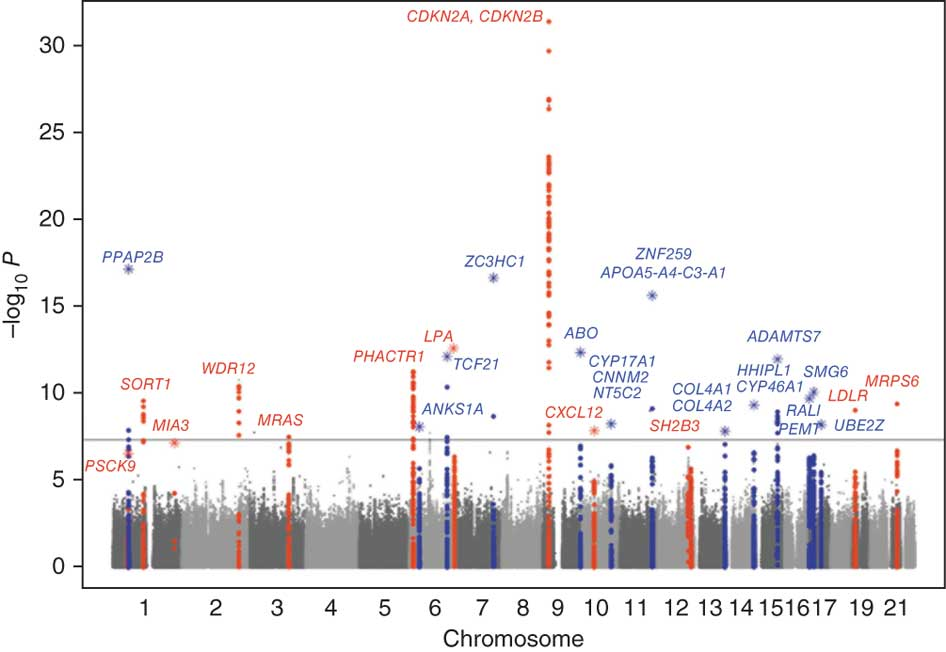
\includegraphics[width=0.5\textwidth]{Figures/man_ex.jpg}
\end{figure}

\subsection{Multiple Comparisson Problem}

In such a set up, where $m$ may be in the millions and the threshold of significance is set to $P = \alpha = 0.05$, we encounter a canonical issue in statistical inference. Recall that $P$ is the probability of observing a $\chi^2$ statistic as large or larger than a specific $\chi^2_m$ assuming $H_0$ of no association is correct and $\alpha$ is the threshold at which a significant effect is declared. Table \ref{hyptest} introduces relevant notation for this section. 


\begin{table}[H]
\centering
\caption{Notation relating to hypothesis testing. Adapted from \cite{Sun2006}}
\label{hyptest}
\begin{tabular*}{.8\linewidth}{@{}llll@{}}
\toprule
                                  & \textbf{True $H_0$} & \textbf{True $H_1$} & \textbf{Total} \\ \midrule
\textbf{Declared significant}     & $V$                 & $S$                 & $R$            \\
\textbf{Declared non-significant} & $U$                 & $T$                 & $m - R$        \\
\textbf{Total}                    & $m_0$               & $m - m_0$           & $m$            \\ \bottomrule
\end{tabular*}
\end{table}


For the sake of description, we define $M$ as the number of \textit{independant} variants (that is, the effective number of variants which are not in \ac{LD} for a given $R^2$ or $D'$ threshold) for sake of description. Thus, $M$ tests and corresponding $M$-vector of $P$ values $\underline{\mathbf{P}}$ is constructed. Because in any statistical test, assuming that $H_0$ is true, there is $\alpha$ chance of falsely rejecting $H_0$ (type I error), by increasing the number of simultaneous tests conducted, the probability of falsely rejecting $H_0$ compounds exponentially as a function of the number of independent test conducted. That is, the conditional probability of falsely rejecting $H_0$ for all $M$ tests may be written as 

$$ Pr(P \leq \alpha \, | \, H_0) = 1-(1 - \alpha)^M $$

This may equivalently be described as the probability of making at least one false positive in $M$ tests. This may alternatively be notated 

$$ Pr(V \geq 1) = 1-(1 - \alpha)^M $$

Speaking asymptotically, $\lim_{M \to \infty} 1-(1 - \alpha)^M = 1$ and false positves are guarenteed. It is against this backdrop that we recall in any relevant genetic context, $M$ is large, and false positives are almost guarenteed.

There exist several ways to correct for this issue, chief among them is the widely adopted Bonferroni correction. Put simply, Bonferroni correction adjusts testing such that $Pr(V \geq 1) = \alpha$ rather than $1-(1 - \alpha)^M$. It does so by rejecting all tests $p_i \in \underline{\mathbf{P}} | i \in 1 \dots M, i \in \mathbb{Z}^+$ such that

$$ p_i \leq \frac{\alpha}{M} $$


The proof is not complex, but shall not be presented here for the sake of brevity. [cite bf]  This adjustment (for $Pr(V \geq 1)$) is defined as control of the \ac{FWER}. This approach does not make any assumptions about the internal dependency strucutre of the tests, and as such, is conservative in the case of all categories of dependency. This is often undesired, as typically researchers will not prune their \ac{GWAS} data to only independant variants. A more commonly accepted procedure, controlling the \ac{FDR} rather than the \ac{FWER} adjusts $\underline{\mathbf{P}}$ such that the proportion of false disoveries in all discoveries is controlled at $\alpha$: 

$$ FDR \equiv E \left[ \frac{V}{R} \right] = \alpha $$

This approach has the benefit of being adaptable and more powerful in circumstances of some forms of dependency (most notably \ac{PRDS} which is common scenario) and is most often applicable to \ac{GWAS} where researchers are more willing to find more true positives at the cost of a fraction of false positives.

Therefore, in summation, \ac{GWAS} is a statistical investigation which estimates several parameters given certain assumptions. Concepts presented in this section will be important background knowledge for the following sections, as most of our model builds off of these premeses. 

\section{Polygenic Prediction of Complex Disease}

Refering to the defintions proposed in the previous section and recalling that in a general additive model, a phenotype vector $\underline{\mathbf{Y}}$ may be expressed as a linear combination of the $\underline{\beta}$ weighted genetic $n \times m$-matrix $\mathbf{G}$ and $\underline{\epsilon}$ following a standard normal $N(0, 1)$ distrbution: 

$$ \underline{\mathbf{Y}} = \underline{\beta}' \mathbf{G} + \underline{\epsilon} $$

It has been previously proposed to combine genetic variants in order to crease a score $S$ which encompases estimated genetic effects in order to predict the phenotype vector $\underline{\mathbf{Y}}$. Define $S$ for individual $n$:

$$ S_n = \sum^m_{i=1} \beta_i G_{ni} $$

Note that in practice, our true statistics must be estimated. The logical estimator of $\underline{\beta}$ is the ordinary least squares regression estimator $\hat{\beta}$. There are other estimators, but the remainder of this section assumes this estimator. Our score is therefore described as:

\begin{equation} 
\label{score}
\begin{aligned}
\hat{S}_n = \sum^m_{i=1} \hat{\beta}_i G_{ni} 
\end{aligned}
\end{equation}

This score has several important properties which will be exploited in the below analysis. Note that in practice, $\underline{\beta}$

Notably, the non-centrality parameter of the $\chi^2$ test for association between $\hat{S}$ and $\underline{Y}$ in the test population, assuming that $\hat{\beta}$ has been estimated in a training population of size $n_1$ and tested in a test population of size $n_2$, is given by:

$$ \lambda = \frac{n_2 R^2_{\hat{S}, Y}}{1 - R^2_{\hat{S}, Y}} $$

Where $R^2_{\hat{S}, Y}$ is the percent explained variance of the phenotype $Y$ with the estimated score $\hat{S}$. 

Additionally, note that $E[\hat{S}] = 0$ and the second moment in a particular individual is given by

$$ \begin{aligned} Var(\hat{S}) &= \sum^m_{i=1} Var(\hat{\beta}_{il}, G_{i}) \\ &= \sum^m_{i=1} \hat{\beta}_{i} \\ &\approx m Var(\hat{\beta}_{i}) \end{aligned} $$

These mathematical properties become important later. These identities have been adapted from \cite{Dudbridge2013}.

\section{Polygenic Sliding Window Optimization}

Frequently, not all $m$ variants are used in the construction of the \ac{PRS} though. Typically, researchers will type the top $m | P_m \leq \alpha_{adj}$ where $\alpha_{adj}$ denotes the shifted acceptance threshold after multiple testing correction. We denote these variants as $m_{P \leq T}$ where $T$ is the $P$ value threshold. 

Though these variants have the highest probability of being truly associated with the phenotype, constructing a score with this few \ac{SNP}s misses the many small and insignificant effects hidden in marginally significant and insignificant hits. Thus, \cite{Euesden2014} have developed a method to find the best-fit \ac{PRS}, that is, the PRS which maximizes genomic signal while minizing noise as in \ref{pt}. We denote this as the \ac{oPRS}. 

\begin{figure}[h]
\label{pt}
\caption{\ac{oPRS} plot for schizophrenia predicting major depresive disorder status. Adapted from \cite{Euesden2014}}
\centering
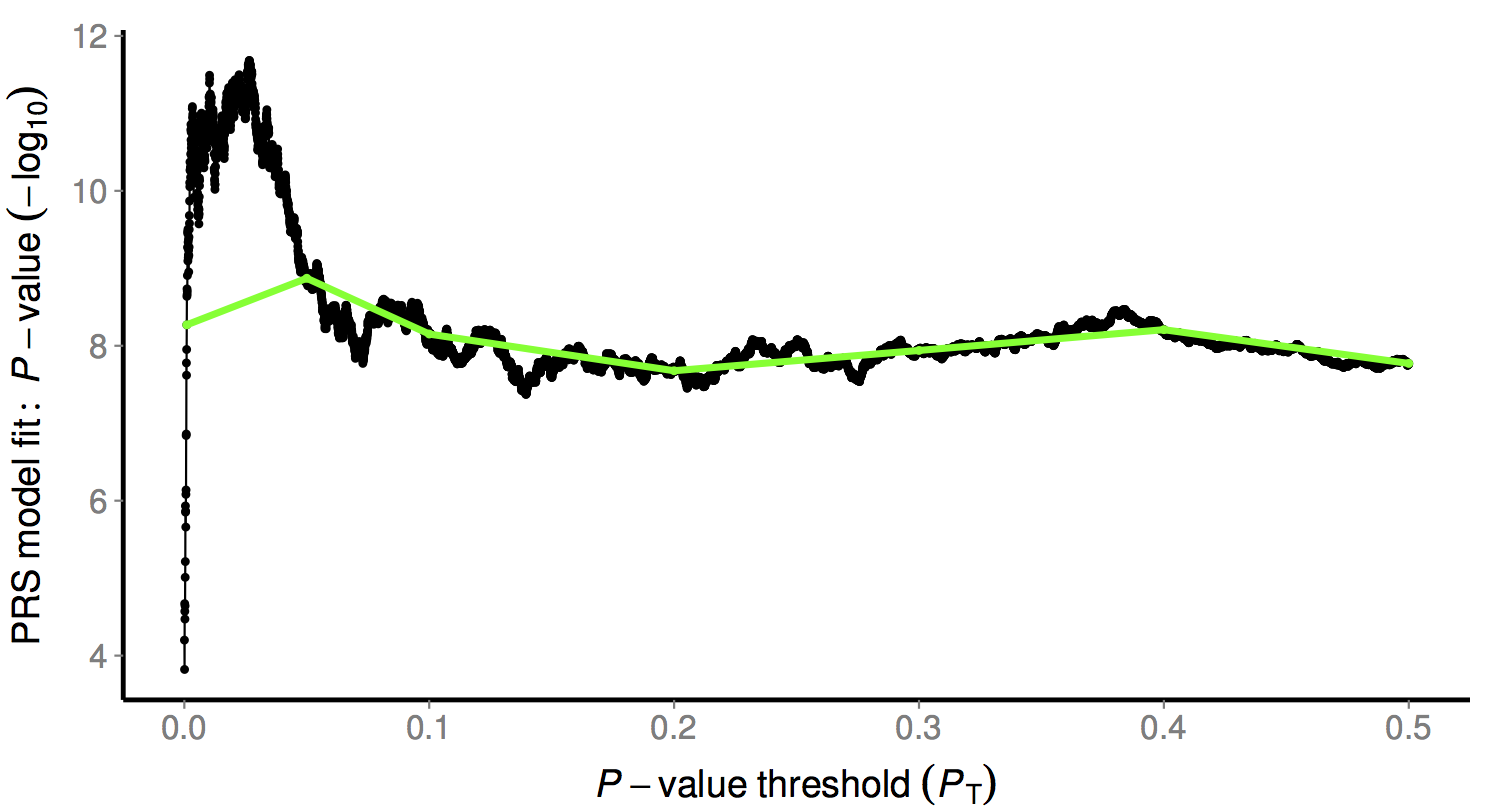
\includegraphics[width=0.8\textwidth]{Figures/pt.png}
\end{figure}

On a high level, this score involves iterating through a list of $P$ value thresholds $T$, constructing a score using all $m_{P < T}$ and selecting either the smallest $P$ value of association between $\hat{S}$ and $\underline{\mathbf{Y}}$ or the highest $R^2_{\hat{S}, Y}$ to move in the analysis. 

More formally, we fix individual $n$ and construct a vector of estimated scores $\underline{\hat{S}}$ with length $n_T$ equal to the number of attempted $P$ value thresholds. 

$$ \begin{aligned} \underline{\hat{S}} &\equiv \begin{bmatrix} \hat{S}_{T_1} \\ \vdots \\ \hat{S}_{n_T} \end{bmatrix} &&&&& \hat{S}_T &= \sum^{m_{P \leq T}}_{i=1} \hat{\beta}_i G_{ni} \end{aligned}$$

Note, however, that when we build a score at each threshold for each individual, an $n \times T$ matrix is constructed, where $n$ is the number of individuals and $T$ is the number of thresholds. The entries are the estiamted score $\hat{S}_{nT}$ for individual $n$ at threshold $T$:

$$ \bold{\hat{S}} = \begin{bmatrix} \hat{S}_{1,1} & \dots & \hat{S}_{1, T} \\ \vdots & \ddots & \vdots \\ \hat{S}_{n, 1} & \dots & \hat{S}_{n, T} \end{bmatrix} $$

\section{Summary}